\subsection{Architecture}
\label{subsec_method_architecture}

The architecture of \emph{Match Forrest, Match!} is shown in Figure \ref{fig_architecture}.


The central component of the system is the \textit{Task Distributor}.
This component is responsible for managing the other components, \textit{Crawler}, \textit{Triplifier}, \textit{Updater} and \textit{Matcher and Merger}.
The details of this messaging systems are explained in Section \ref{subsubsec_messaging_infrastructure}.


In general the first step to get a movie into the system, is to get the acutal movie resource.
This step is done by the \textit{Crawler.}
This component is responsible to download websites or to send a request to the provided API from a data source.

Once the page is downloaded, the \textit{Triplifier} can triplify the resource.
This means it takes the information from the resource and creates triples out of it.
Therefore, the ontology, defined in Section \ref{subsec_method_ontology}, is used.

The component \textit{Matcher and Merger} is in charge of matching two movies from different data sources, so they only can be found once in the resulting dataset.
This component is explained in detail in Section \ref{subsec_method_matching}.

The updater, described in Section \ref{subsec_method_updating}, ensures that the movies are always up to date.

The triplestore \textit{Virtuoso} is used, to store the resulting triples.
To distinguish between the sources of the different triples, triples from one datasource are stored in the same graph named after the resource.
So, there are four graphs in the triplestore, \textit{imdb}, \textit{freebase}, \textit{tmdb} and \textit{ofdb}.

\begin{figure}[ht]
  \begin{center}
  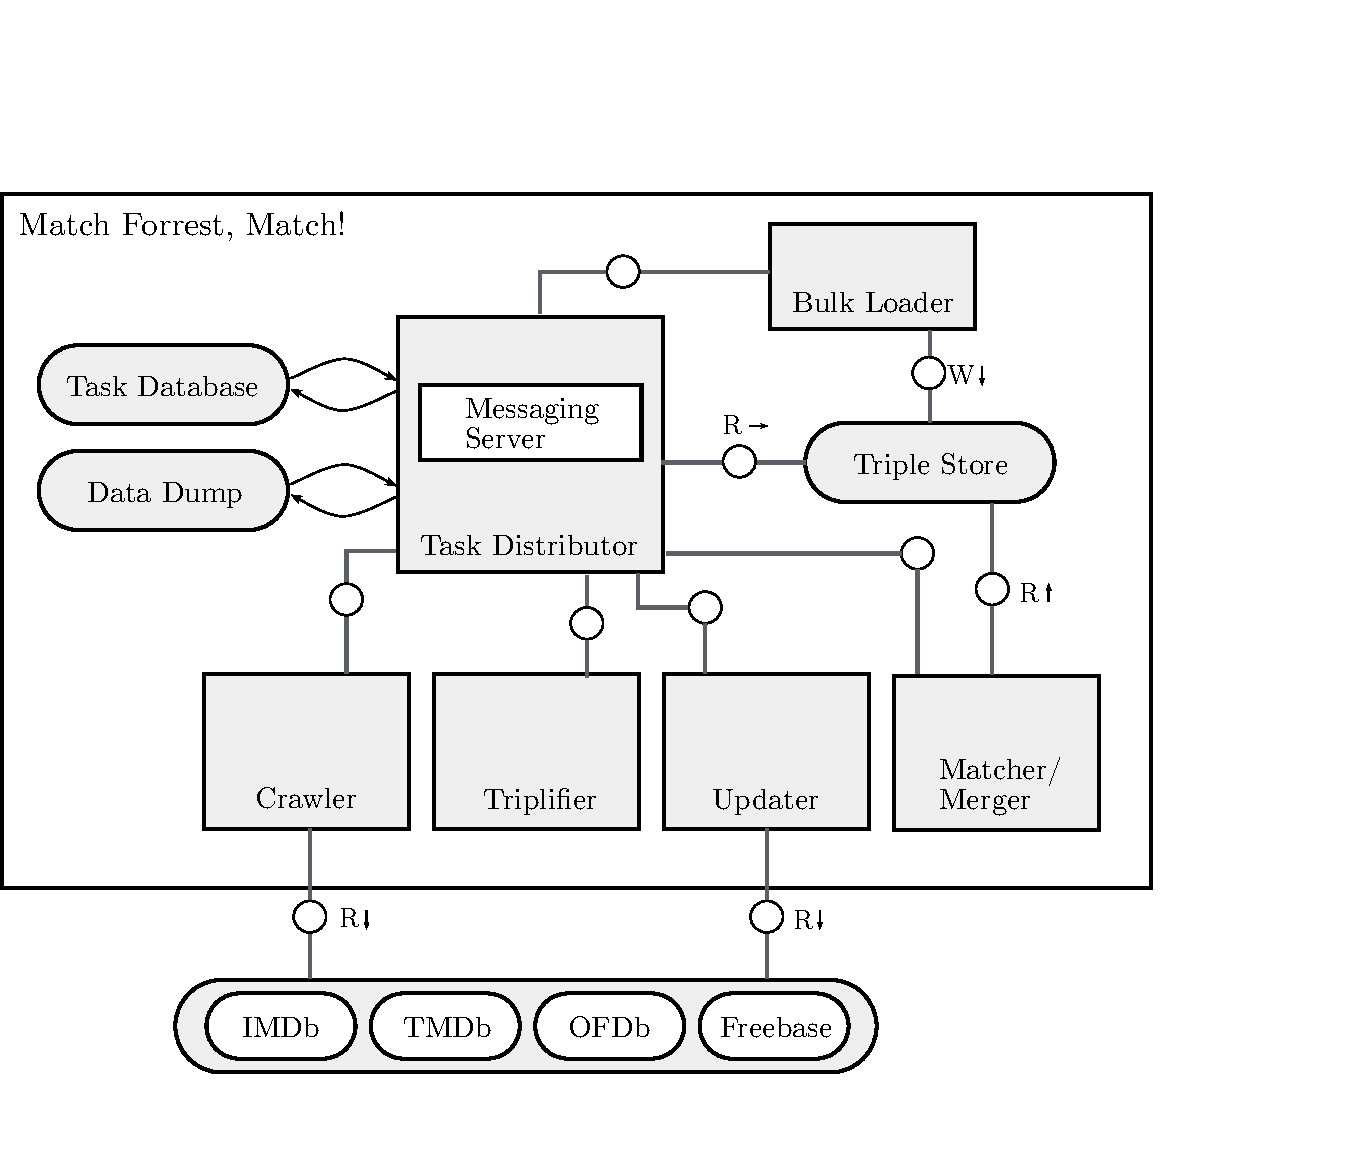
\includegraphics[width=0.5\textwidth]{images/architecture.pdf}
  \end{center}
  \caption{Architecture}
  \label{fig_architecture}
\end{figure}

\subsubsection{Messaging Infrastructure}
\label{subsubsec_messaging_infrastructure}

\begin{figure}[ht]
  \begin{center}
  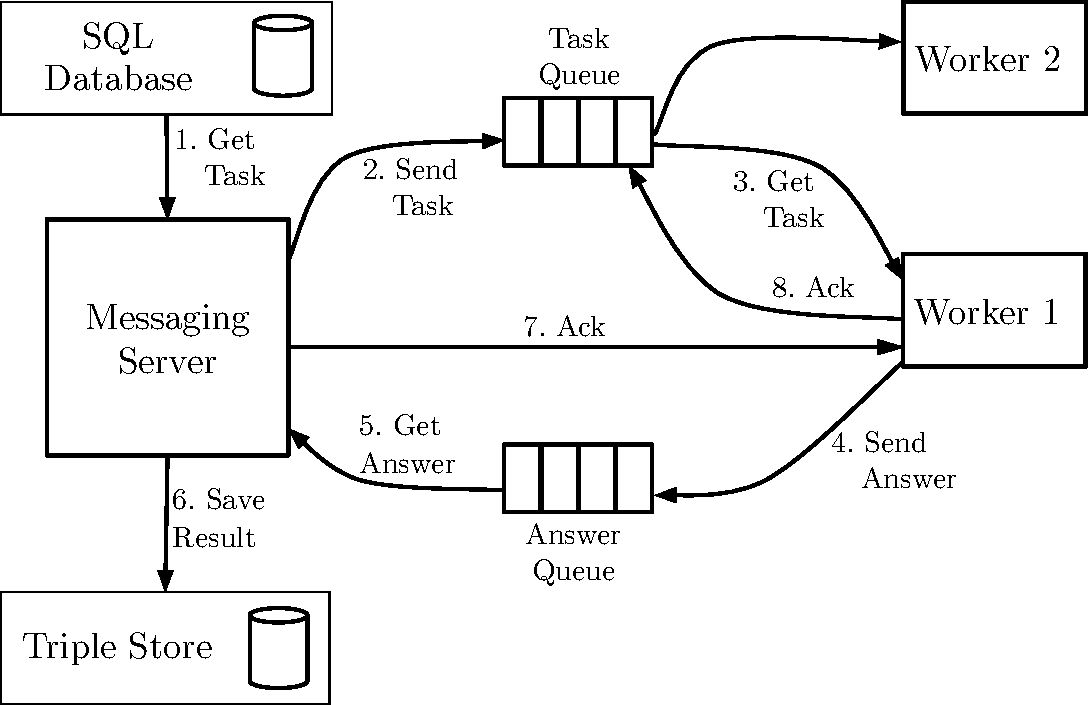
\includegraphics[width=0.5\textwidth]{images/rabbit_mq.pdf}
  \end{center}
  \caption{Messaging Infrastructure using RabbitMQ}
  \label{fig_messaging_infrastructure}
\end{figure}